\documentclass[tikz,border=8pt]{standalone}
\usepackage{amsmath,amssymb}
\usetikzlibrary{arrows.meta,calc}

\begin{document}
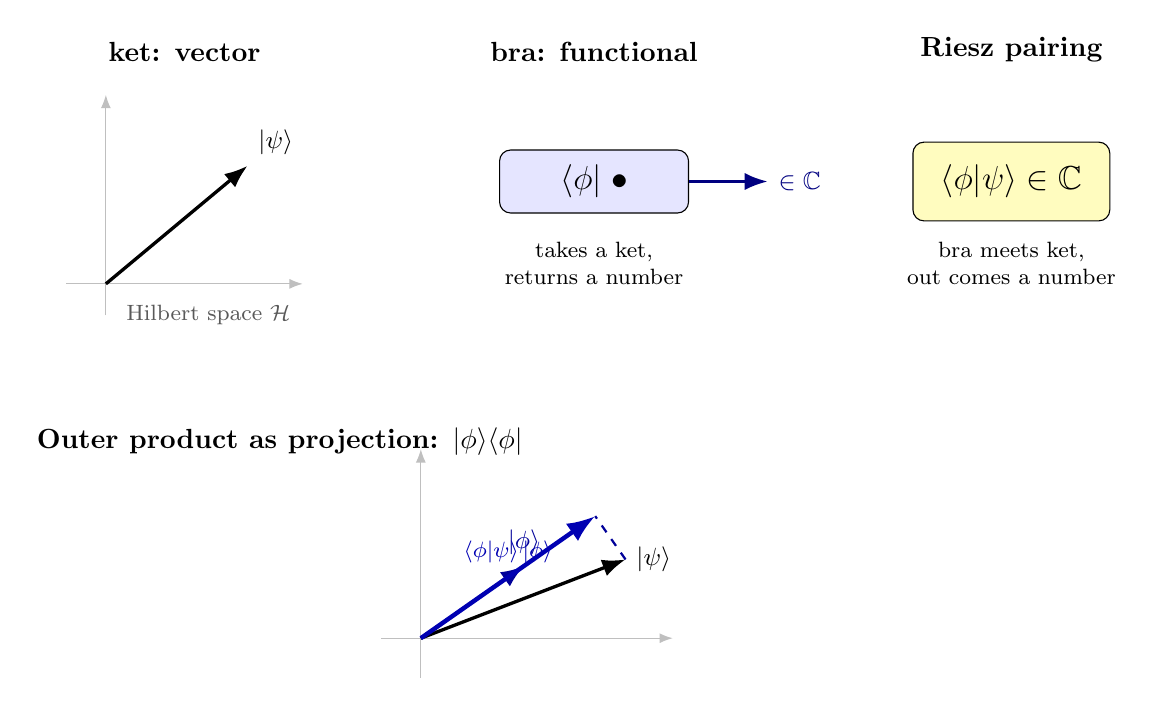
\begin{tikzpicture}[>=Latex]

  % TOP-LEFT: ket as vector
  \begin{scope}[xshift=0cm, yshift=0cm]
    \node[font=\bfseries, anchor=south] at (1.0, 2.7) {ket: vector};
    \draw[->, thin, gray!50] (-0.5, 0) -- (2.5, 0);
    \draw[->, thin, gray!50] (0, -0.4) -- (0, 2.4);
    \draw[->, very thick, black] (0, 0) -- (1.8, 1.5) node[above right, font=\small]{$|\psi\rangle$};
    \node[font=\footnotesize, gray!70!black] at (1.3, -0.4) {Hilbert space $\mathcal H$};
  \end{scope}

  % TOP-MIDDLE: bra as functional
  \begin{scope}[xshift=4.7cm, yshift=0cm]
    \node[font=\bfseries, anchor=south] at (1.5, 2.7) {bra: functional};
    \node[draw, fill=blue!10, rounded corners, minimum width=2.4cm, minimum height=0.8cm, font=\large] (br) at (1.5, 1.3) {$\langle\phi|\;\bullet$};
    \draw[->, very thick, blue!50!black] (br.east) -- ++(1.0, 0) node[right, font=\small]{$\in\mathbb C$};
    \node[font=\footnotesize, anchor=north, align=center] at (1.5, 0.65) {takes a ket,\\returns a number};
  \end{scope}

  % TOP-RIGHT: pairing
  \begin{scope}[xshift=10cm, yshift=0cm]
    \node[font=\bfseries, anchor=south] at (1.5, 2.7) {Riesz pairing};
    \node[draw, fill=yellow!25, rounded corners, minimum width=2.5cm, minimum height=1.0cm, font=\large] at (1.5, 1.3) {$\langle\phi|\psi\rangle\in\mathbb C$};
    \node[font=\footnotesize, anchor=north, align=center] at (1.5, 0.65) {bra meets ket,\\out comes a number};
  \end{scope}

  % BOTTOM: outer product = projection
  \begin{scope}[yshift=-4.5cm]
    \node[font=\bfseries, anchor=west] at (-1, 2.5) {Outer product as projection: $|\phi\rangle\langle\phi|$};

    \begin{scope}[xshift=4cm]
      \draw[->, thin, gray!50] (-0.5, 0) -- (3.2, 0);
      \draw[->, thin, gray!50] (0, -0.5) -- (0, 2.4);

      % unit phi
      \draw[->, very thick, blue!60!black] (0, 0) -- ({1.6*cos(35)},{1.6*sin(35)}) node[above, font=\small]{$|\phi\rangle$};

      % psi
      \draw[->, very thick, black] (0, 0) -- (2.6, 1.0) node[right, font=\small]{$|\psi\rangle$};

      % projection foot
      \pgfmathsetmacro{\pp}{2.6*cos(35) + 1.0*sin(35)}
      \pgfmathsetmacro{\px}{\pp*cos(35)}
      \pgfmathsetmacro{\py}{\pp*sin(35)}

      \draw[dashed, thick, blue!60!black] (2.6, 1.0) -- (\px, \py);
      \draw[->, ultra thick, blue!70!black] (0, 0) -- (\px, \py);
      \node[anchor=south, font=\footnotesize, blue!70!black] at ({\px*0.5}, {\py*0.5+0.05}) {$\langle\phi|\psi\rangle\,|\phi\rangle$};
    \end{scope}
  \end{scope}
\end{tikzpicture}
\end{document}
